% file: jupiter-tlaplus-chain.tex
% not finished!!!

\documentclass[tikz]{standalone}
\usetikzlibrary{chains, scopes}

\begin{document}
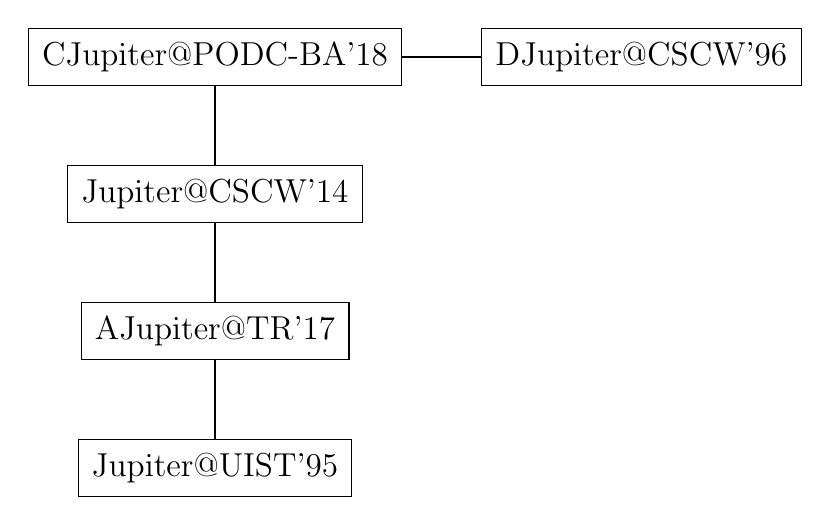
\begin{tikzpicture}[every on chain/.style = {join},
    every join/.style = {-, thick},
    node distance = 1.0cm and 1.0cm,
    every node/.style = {draw, font = \large, inner sep = 5pt}]
  { [start chain = p2p]
    \node (cjupiter) [on chain] {CJupiter@PODC-BA'18};
    { [start branch = cs going below, join = by {blue}] }
    \node (djupiter) [on chain] {DJupiter@CSCW'96};

    { [continue branch = cs]
      \node (xjupiter) [on chain] {Jupiter@CSCW'14};
      \node (ajupiter) [on chain] {AJupiter@TR'17};
      \node (njupiter) [on chain] {Jupiter@UIST'95};
    }
  }
\end{tikzpicture}
\end{document}
